\chapter{Ovládání}
\label{7-aplikace}
Pro ovládání dronu byla vytvořena aplikace pro mobilní operační systém Android. Aplikace byla napsána v programovacím jazyku Java a programovacím prostředí Android studio.\cite{android} \cite{codemitch}\\
Aplikace využívá Bluetooth, GNSS mobilu. Přes bluetooth modul probíhá přenos dat pro ovládání dronu, GNSS slouží pro zjištování polohy uživatele a zobrazení na okně s Google Maps.\\

\section{Hlavní obrazovka}
Při otevření aplikace se na display zobrazí hlavní obrazovka. Zde má uživatel na výběr zda využije manuální či autonomní ovládání. Po rozkliknutí jednoho ze spárovaných bluetooth zařízení, aplikace otevře okno pro ovládání.\\
\begin{figure}[H]
	\centering
	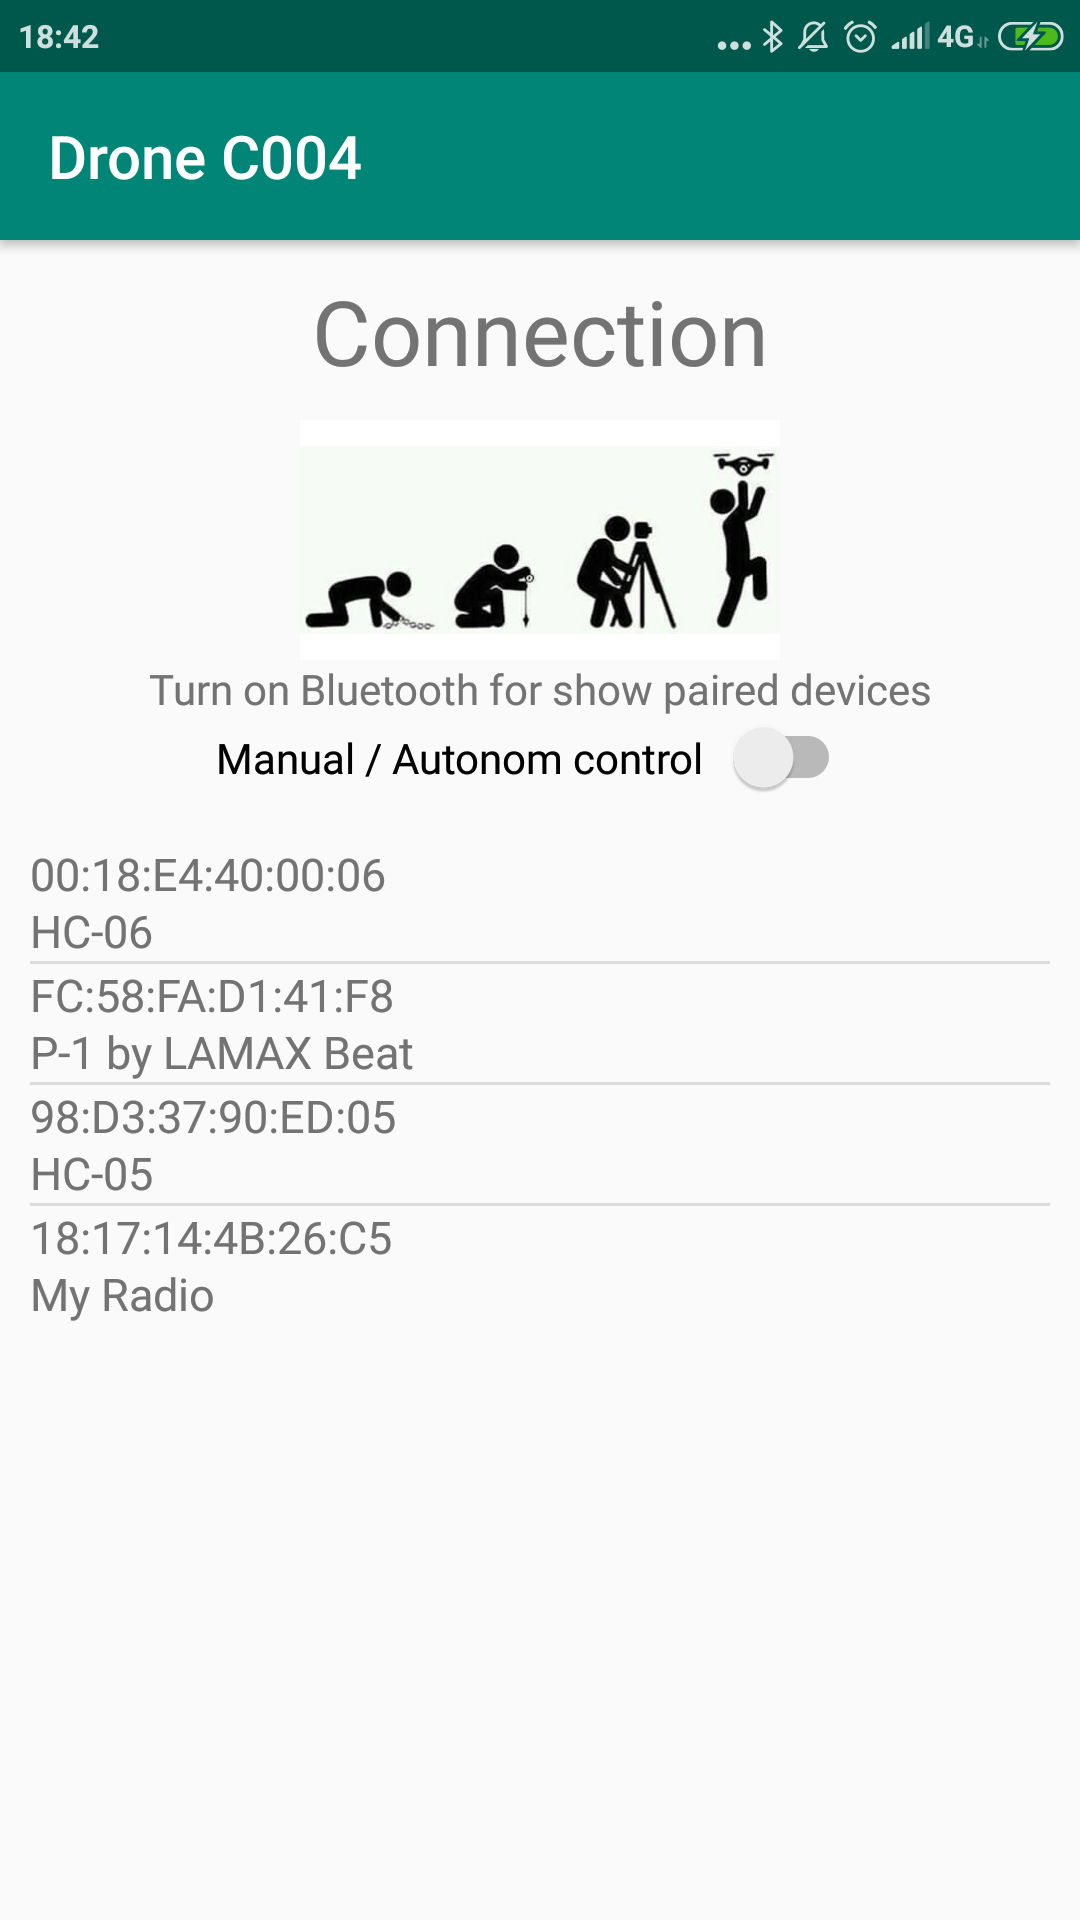
\includegraphics[width=6cm]{pictures/app1.png}
	\caption{Screenshot hlavní obrazovky}
\end{figure}

\section{Manuální ovládání} 
Manuální ovladání funguje totožně jako RC soustava. Levý joystick slouží k ovládání náklonů pitch a roll, pravý joystick složí k ovládání throttle a yaw. Informace o poloze joystiků jsou posílány přes bluetooth komunikaci do uzlového zařízení. Typ zprávy je popsán v kapitole komunikační protokol.\\
Při tvorbě joysticků byla použita knihovna Virtuální joystick, u které byl upraven rozsah snímaných souřadnic ukazatele a definová jiných předávaných parametrů. Předávácí parametry byly nastaveny polární souřadnice, po změně předávají kartézské souřadnice. \cite{joystick}\\\\

\begin{figure}[H]
	\centering
	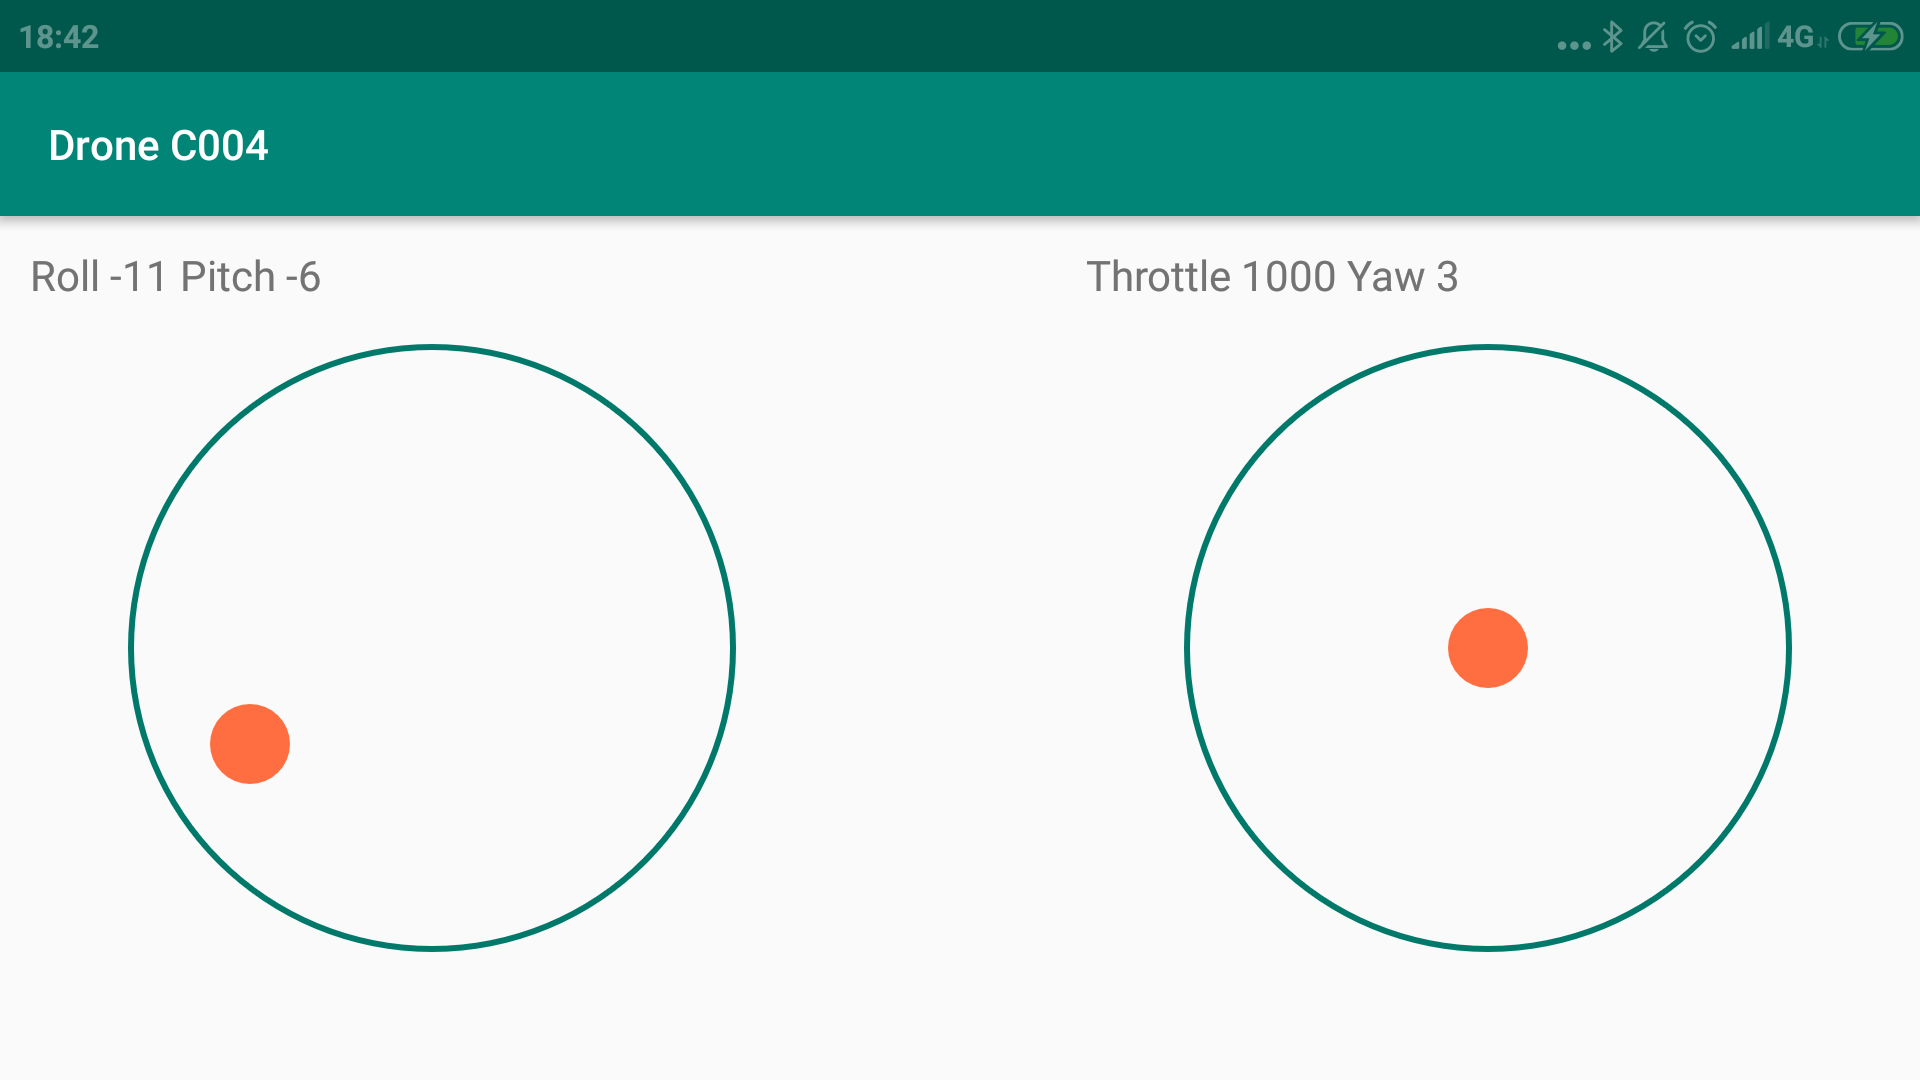
\includegraphics[width=10cm]{pictures/app.png}
	\caption{Schreenshot obrazovky pro manuální ovládání}
\end{figure}

\begin{figure}[H]
	\centering
	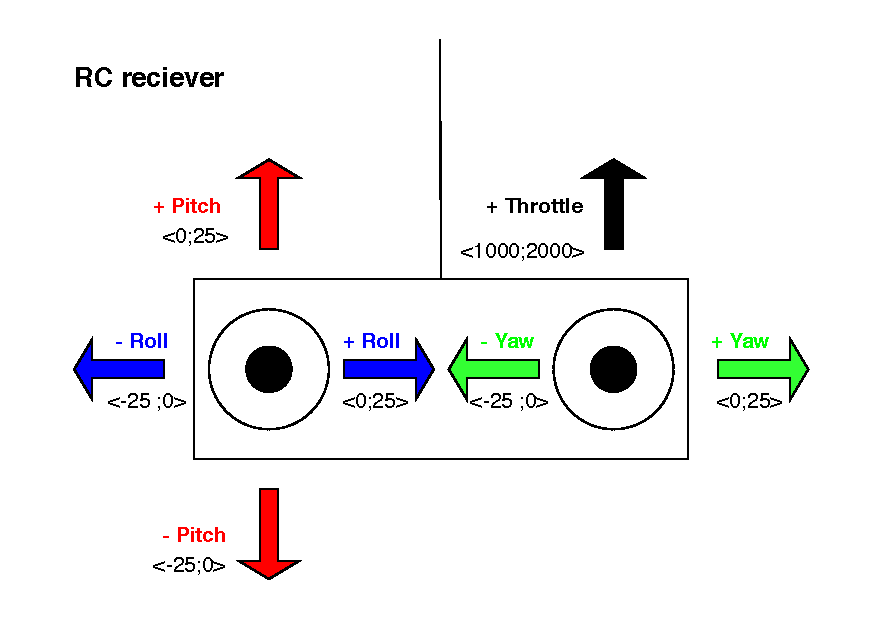
\includegraphics[width=14cm]{pictures/rcDiagram.pdf}
	\caption{Diagram RC soustavy}
\end{figure}

\section{Autonomní ovládání} 
Pro autonomní ovládání stačí pouze zadat souřadnice v systému WGS-84. Přes tlačítko SEND je zaslat dronu a uživatel může na mapě sledovat, kde se dron nachází. Spodní tlačítko Home slouží k návratu dronu a startovní místo. Autonomní ovládání je též ve vývoji, zprovoznění bude možné až po dokončení navigačního kontroléru.\\
Mapa je generována ze servrů Google Maps přes API. API je možné používat po registraci pro google vývojáře a nastavení API pro aplikaci.\\

\begin{figure}[H]
	\centering
	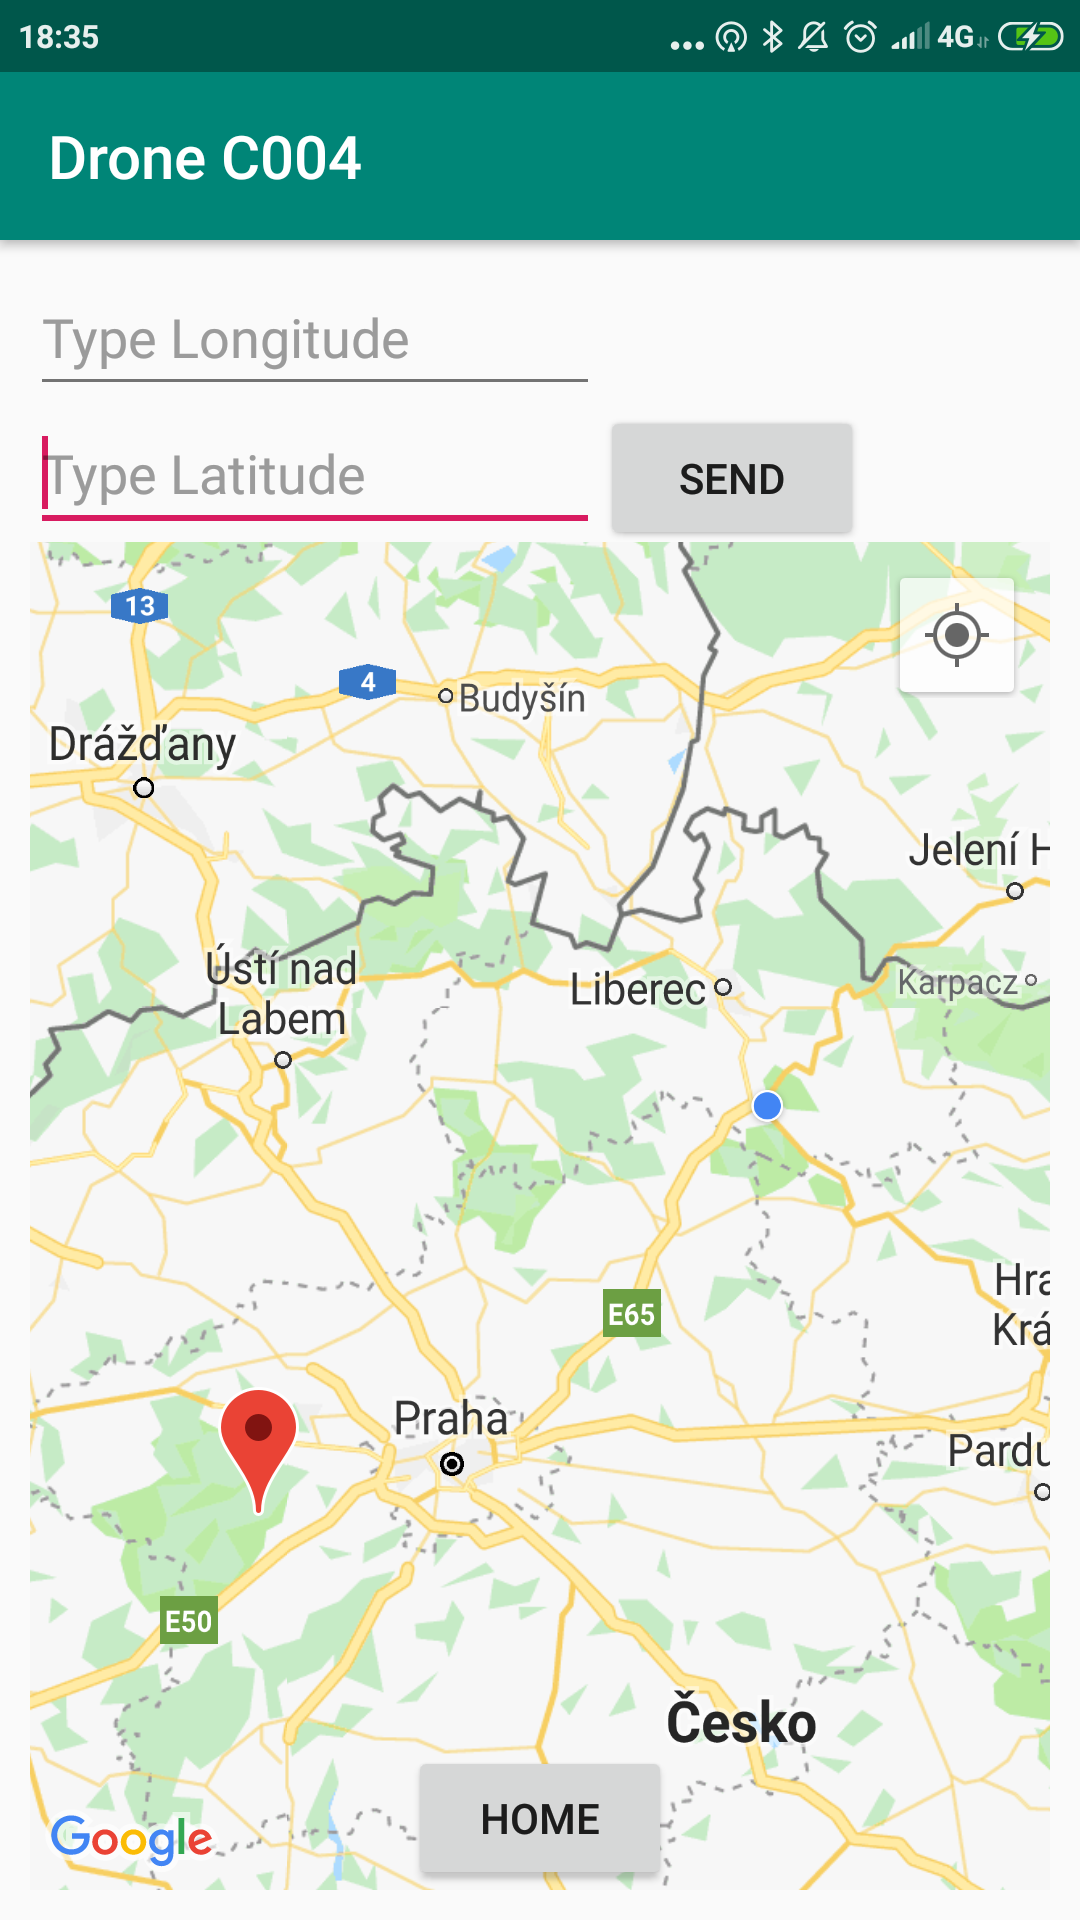
\includegraphics[width=6cm]{pictures/app2.png}
	\caption{Schreenshot obrazovky pro autonomní ovládání}
\end{figure}

\section{Kamera}
Bylo v plánu implementovat obraz z kamery z dronu do mobilní aplikace. Bohužel pro nedostatku času a málo zkušeností s Android studiem je tato část pouze rozpracovaná. Pro zobrazení obrazu v aplikace byla použita více platformové knihovny libusb a libuvc.\\
Obraz z kamery lze sledovat přes mobilní aplikaci FPViewer. Po zapojení přijímače obrazového signálu se aplikace automaticky zapne.\\

\begin{figure}[H]
	\centering
	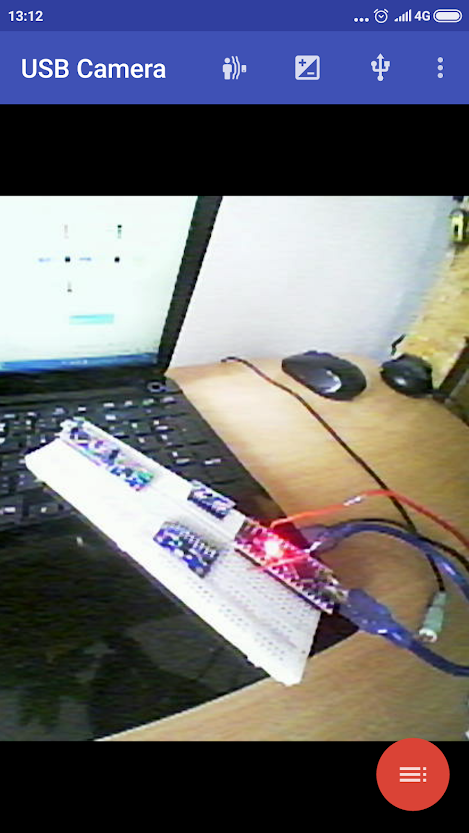
\includegraphics[width=6cm]{pictures/fpvscreenshot.png}
	\caption{Schreenshot aplikace FPViewer}
\end{figure}

